\documentclass[times]{article}

\usepackage{graphicx}
\usepackage{float}
\usepackage{placeins}
\usepackage[none]{hyphenat}
\usepackage{amsmath}
\usepackage[us]{datetime}
\usepackage[explicit]{titlesec}
\titleformat{\section}{\normalfont}{}{0em}{\textbf{\large Problem  \thesection}\  \normalsize #1}
\begin{document}
	\title{CS 5800 Distributed OS - Spring 2017 \\ Homework 5}
	\author{Josh Herman \\ Dalton Cole \\ Neil Blood}
	\date{\formatdate{27}{4}{2017}}
	\maketitle

	% Problem 1
	\section{Assuming that the communication network is synchronous, does the proposed algorithm work? If not, provide an example where there are at least 2 traitors.}
		Let the default be 1 when a tie is reached and let the commander and lieutenant 6 be traitors. After tracing the tree, shown in Figure 1, it can be seen that lieutenant 1 would receive: (0,1,0,1,0,0) giving a majority value of 0, lieutenant 2 would receive: (1,0,0,1,0,1) giving a tie so going with the default of 1, lieutenant 3 would receive: (0,0,1,1,0,0) giving a majority value of 0, lieutenant 4 would receive: (1,0,1,0,0,1) giving a tie so going with the default of 1, and lieutenant 4 would receive: (0,0,1,0,1,0) giving a majority value of 0. Since the lieutenants do not all reach the same decision the proposed algorithm does not work.
		
		\begin{figure}[H]
			\caption{Problem 1}
			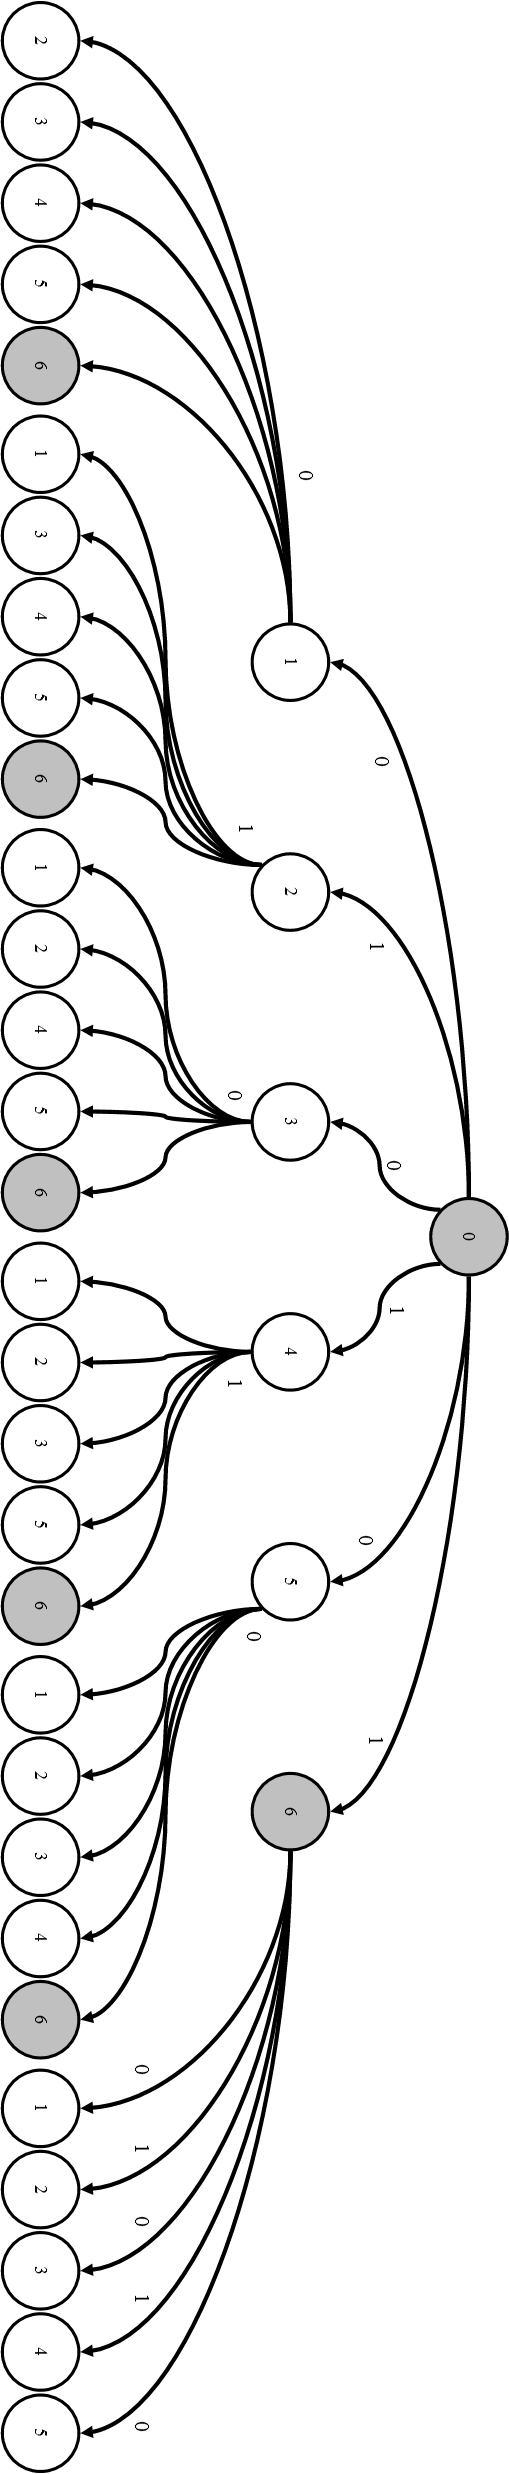
\includegraphics[height=\textheight]{q1.png}
		\end{figure}
	
	% Problem 2
	\section{Using the same example, show, step by step, how Lamport’s algorithm allows the generals to reach an agreement.}
		Let the default be 1 when a tie is reached and let the commander and lieutenant 6 be traitors. After tracing the tree, shown in Figure 2, it can be seen that lieutenant 1 would receive: (1,0,1,0,0) giving a majority value of 0, lieutenant 2 would receive: (0,0,1,0,1) giving a majority value of 0, lieutenant 3 would receive: (0,1,1,0,0) giving a majority value of 0, lieutenant 4 would receive: (0,1,0,0,1) giving a majority value of 0, and lieutenant 4 would receive: (0,1,0,1,0) giving a majority value of 0. Following the algorithm all of the loyal generals were able to successfully reach an agreement of 0.
		
		\begin{figure}[H]
			\caption{Problem 2}
			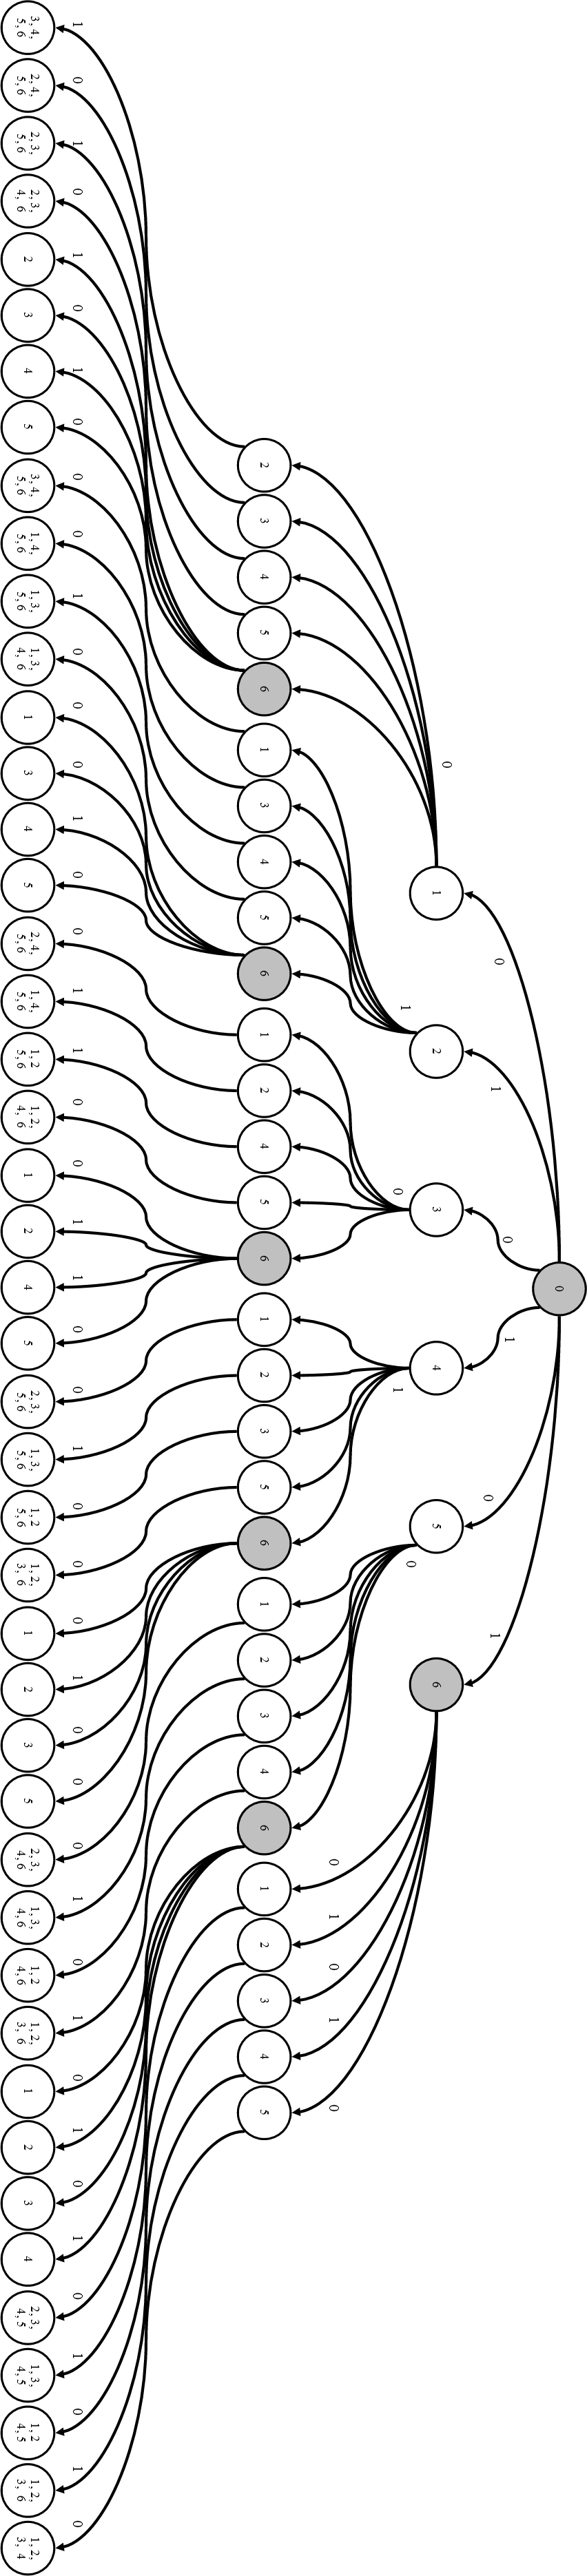
\includegraphics[height=\textheight]{q2.png}
		\end{figure}
	% Problem 3
	\section{Suppose there are k traitors among n generals, calculate the number of messages sent by a lieutenant under the Lamport’s algorithm.}
		If there are k traitors and n generals, then the message complexity will be bounded by $O(n^{k+1})$ with an exact count of messages sent being:

		\begin{equation*}
			\sum_{i=1}^{k+1} \frac{(n-1)!}{(n-1-i)!}
		\end{equation*}

		This is because, for the first row, or stage, $(n-1)$ messages are sent, as seen in question 2. In the second row, $(n-1)*(n-2)$ messages are sent. This pattern continues until the $k^{th} + 1$ row, which is: $(n-1)*(n-2)...(n-(k+1))$. To get total message complexity, we must sum all of these stages, which results in the aforementioned equation.
	

	
	
		
\end{document}